% \part{Experiment}\label{part:experiment}
\chapter{Preparation, manipulation, and measurement of neutral atom qubits}\label{ch:qubit_prep}

\section{MOT}
% finding the "first" MOT, with Z beams at the angle we use.
% say things about the typical size of the MOT, include pictures
% of bright MOTs we've gotten. alignment of the z beams to the 
% repump. signal of the MOT with the SPCM vs magnetic field 
% parameters? reference a figure of the switchyard schematic, which
% we can put in the lasers section
\subsection{Alignment and imaging}

Laser cooling and spatial confinement of atoms in a MOT is the first step in preparing neutral atom qubits, as individual atoms can then be trapped from the cloud of cold atoms in the MOT. The network experiment MOTs are loaded from a background vapor from a Rb ampoule with a naturally occurring isotope ratio.

The first MOT found in network Node 1 used external MOT beams which were perpendicular to the chamber windows for ease of alignment. However, future experiments including atom arrays and Rydberg excitation may require the use of an external objective lens, so we
send the external beams in at an angle of $35^{\circ}$ to the normal to bypass this objective. This reduces complications which would arise from sending the external MOT beams through the same path used for imaging array atoms through the objective, such as heating due to the inability to have three-dimensional cooling while imaging\footnote{Thanks to Trent Graham for useful discussion on this point.}. We note that there are ways to mitigate this kind of issue, but they are often atomic species dependent\cite{covey20192000}.

The alignment of the external MOT beams to those on-chip is necessary to form a MOT,
but tricky due to the lack of optical access from the side of the chamber. Alignment is additionally complicated due to severely limited clearance ($\leq$ 1 mm) at the edge of the 0.4 NA objective lens (custom, JenOptik) mounted at the bottom chamber window. This limitation is shown clearly in Fig. \ref{fig:chamber_cross_section}
\begin{figure}[!ht]
    \centering
    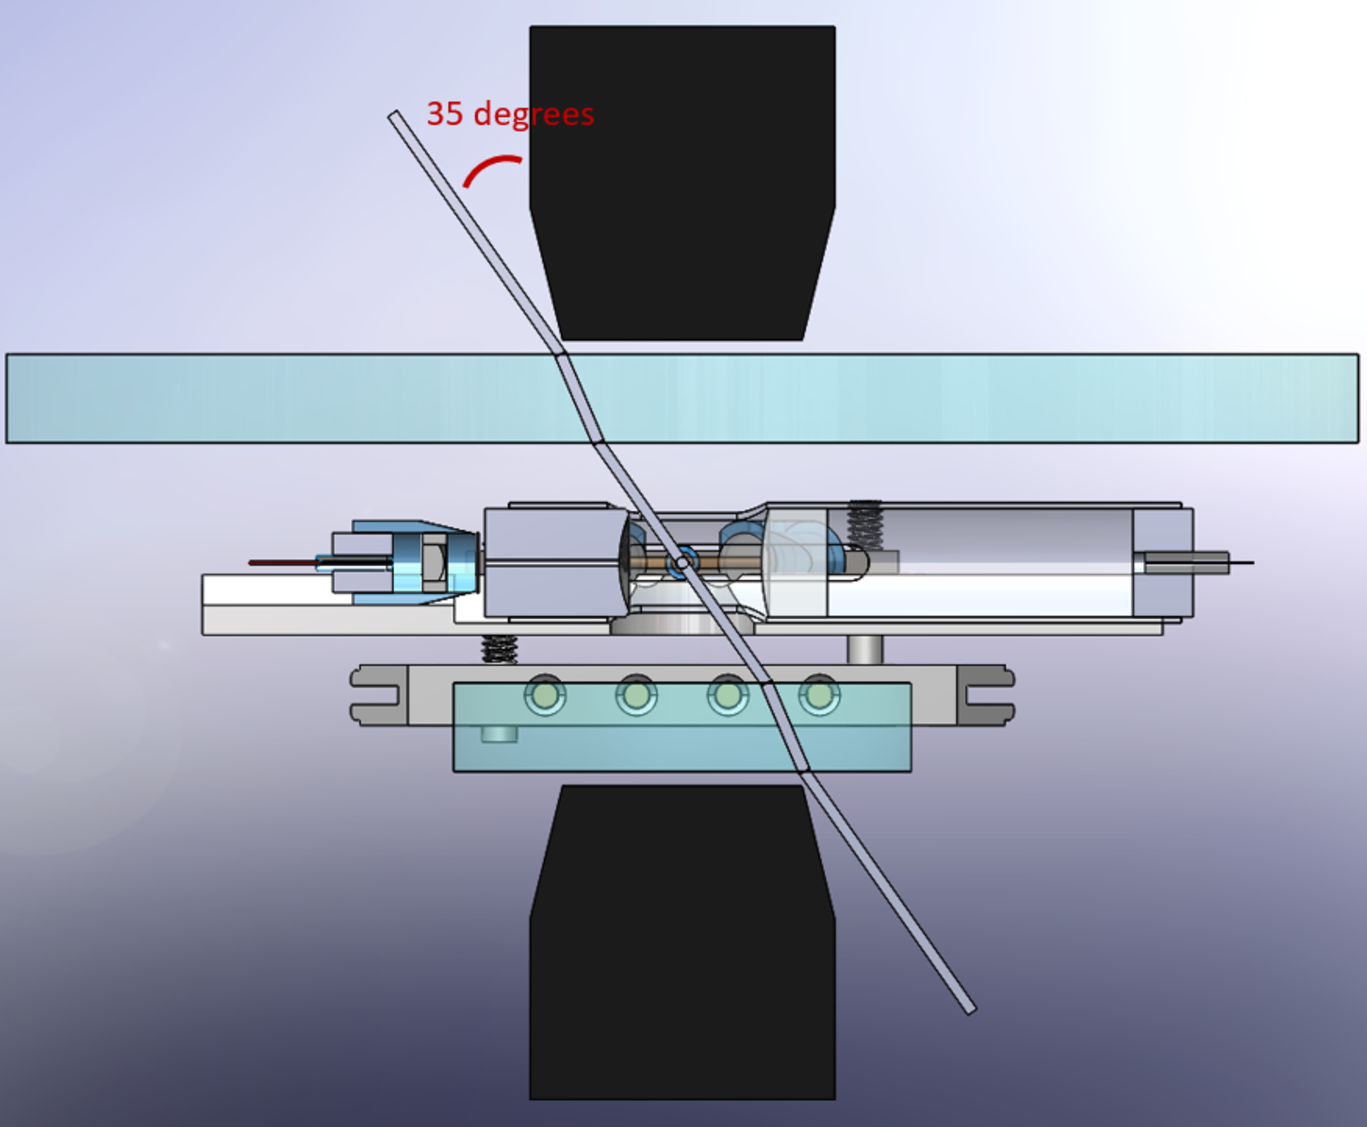
\includegraphics[width=0.9\textwidth]{Images/chamber_cross_section.pdf}
    \caption{Cross section of the network node science chamber, with the steel chamber hidden, with two 0.4 NA JenOptik objectives represented in black. The cylindrical solids representing the MOT beam have radius equal to the $1/e^2$ intensity waist $w_0$, and there is $\sim2w_0$ from the beam axis to the objectives at closest approach.}
    \label{fig:chamber_cross_section}
\end{figure}
We overcame the limitation of optical access by using the atomic fluorescence to verify proper MOT beam alignment. By launching resonant MOT repump light through one of the on-chip MOT beams, and sending only cooling light through the top external MOT beam, we were able to align the top MOT beam until there was an obvious increase in fluorescence where the beams overlapped, as seen by imaging with an Andor Luca camera from the top chamber window\footnote{Better SNR can be acheived using $^{85}\text{Rb}$ transitions as there is more than 2.5 times as much of this isotope compared to $^{87}\text{Rb}$. As our frequency shifting AOMs are not tuned for this isotope, we lock the cooling laser to $^{85}\text{Rb}$'s $\text{D}2$ line cycling transition and tune the repump frequency until we see an increase in fluorescence.}. For this technique to be reliable, it is necessary to make sure there is negligible fluorescence from the repump itself, which would result in an increased fluorescence signal near the overlap region even if the beams are not crossing. The camera settings must also be adjusted to clip the image so background, e.g. from scattering in the chamber, does not obscure the signal. The beam overlap can then be clearly verified by moving the repump on and off resonance, as shown in Fig. (\ref{fig:external_beam_alignment}).
\begin{figure}[!ht]
    \centering
    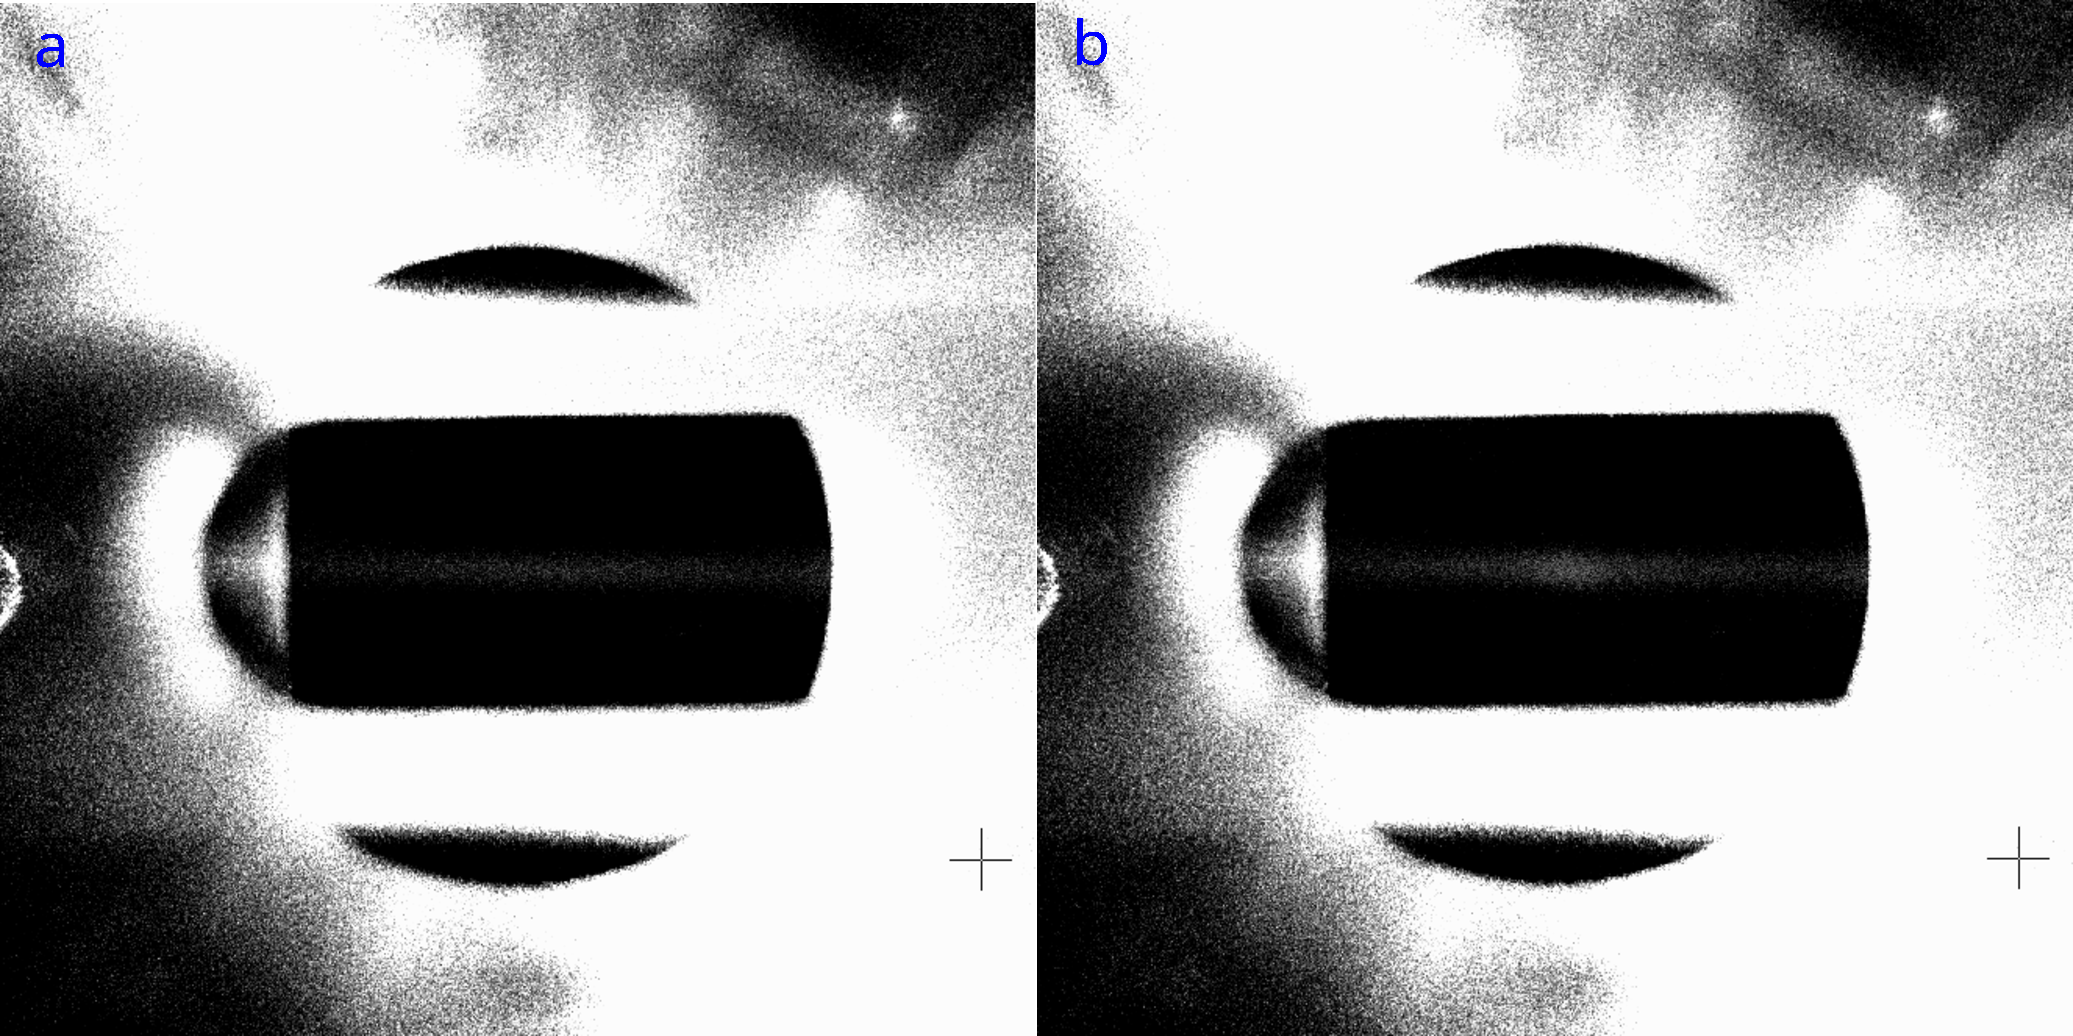
\includegraphics[width=0.9\textwidth]{Images/mot6_alignment_to_repump.pdf}
    \caption{Alignment of the MOT6 beam, containing only cooling 
    light, to an on-chip beam containing only MOT repump light. When the 
    beams are overlapped and the cooling laser is locked as in (b) there is a clear enhancement of the fluorescence in the region of overlap, compared with the case in which the cooling laser is unlocked, shown in (a).}
    \label{fig:external_beam_alignment}
\end{figure}
The bottom external beam can then be aligned to overlap the top beam, for example by coupling it into the top beam fiber. Finally, two things are important to note regarding this alignment procedure. 1) While we were able to find single atoms with less systematic methods of beam alignment, such as sending the beams through the chamber so that they nearly clipped on either edge of the mirror tube, the method described here is the only one which has proven to be repeatable. 2) For good atom loading, we have always needed to slightly misalign the external beams with respect to each other. This is an argument against gluing them in place along with the other beams in a future build.
\begin{figure}[!ht]
    \centering
    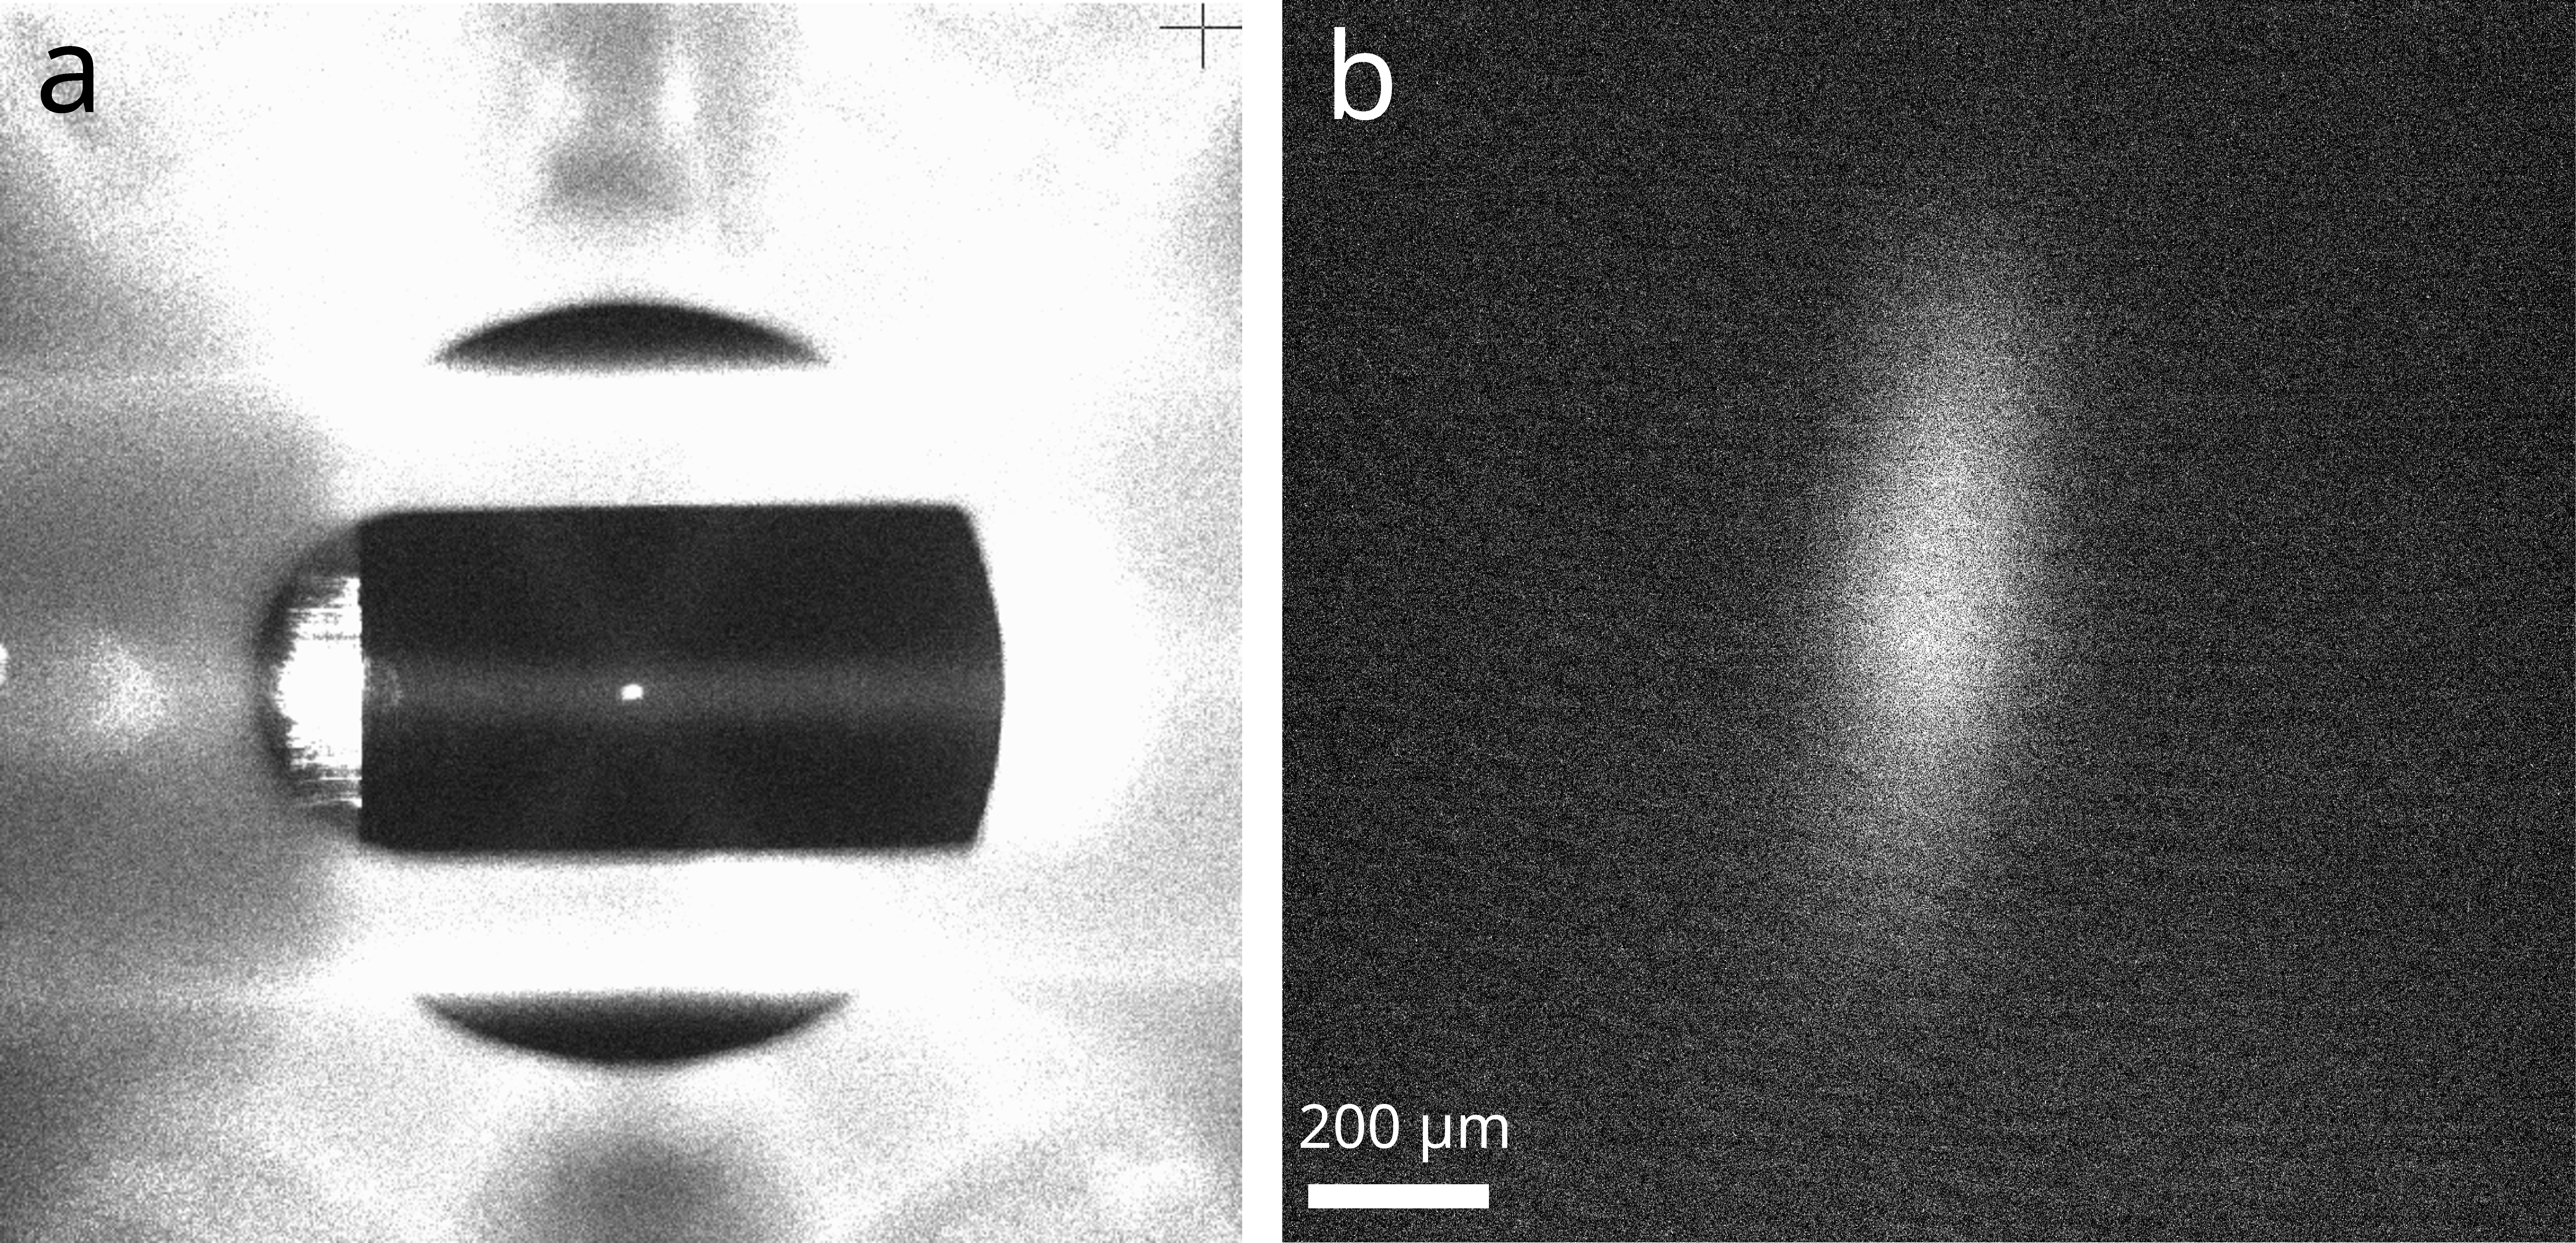
\includegraphics[width=0.9\textwidth]{Images/large_mot_and_thorcam_mot.pdf}
    \caption{(a) A bright MOT captured with Andor Luca, and (b) a more typical MOT 
    as imaged through a custom 0.4 NA objective onto a 
    CS165MU ThorCam.}
    \label{fig:large_mot_and_thorcam_mot}
\end{figure}
An example of a particularly bright MOT is shown in Fig. (\ref{fig:large_mot_and_thorcam_mot}), with a more typical MOT imaged through the bottom objective and 200 mm lens onto a ThorCam CS165MU. The width is about $180~\mu$m in one direction and around twice this in the other. Early measurements of the MOT temperature were done using the time of flight (ToF) technique and the Luca camera imaging through the top window with a zoom lens, giving temperatures around 100 $\mu$K for each axis. However, typically the MOT corresponding to good atom loading is too weak to do ToF imaging with the top camera, and the bottom imaging system has too small a field of view.

\subsection{Fiber AOMs and cooling light power stabilization}\label{sec:fiber_AOM_power_stabilization}

Making sure that the MOT position does not drift over time is crucial for reliable atom loading, especially with a small MOT. One source of instability comes from standing waves between pairs of MOT beams which shift as the phase of the laser varies, causing the MOT to move around. We mitigate this effect by using one fiber AOM for each MOT beam to impart a relative frequency shift of $\sim 10$ kHz between any given pair of beams. It can be shown that for $780$ nm light, this corresponds to 5000 intensity waves (with $\lambda=390$ nm) passing through the MOT in a 0.5 s loading period. 

A second source of instability comes from power imbalance between the pairs of MOT beams, which can also cause variations in MOT temperature. To mitigate this, we employ a DC feedback loop in which the powers of the MOT beams are measured and the corresponding fiber AOMs are used as variable optical attenuators by varying the RF driving power. For the external MOT beams, the power for each beam is measured with a pick-off to a photodiode and transimpedance amplifier\cite{Ebert2017thesis} which comes after the polarization optics but precedes the final mirrors before the chamber. For the on-chip beams, the situation is more complicated. In order to have a reliable measure of the optical power at the atoms, we measure light which couples from one beam (e.g. 2) into the opposite beam's fiber (e.g. 4) in the chamber, with a free space $30:70$ non-polarizing beamsplitter outside of the chamber, as shown in Fig. \ref{fig:mot_feedback}. 
\begin{figure}[!ht]
    \centering
    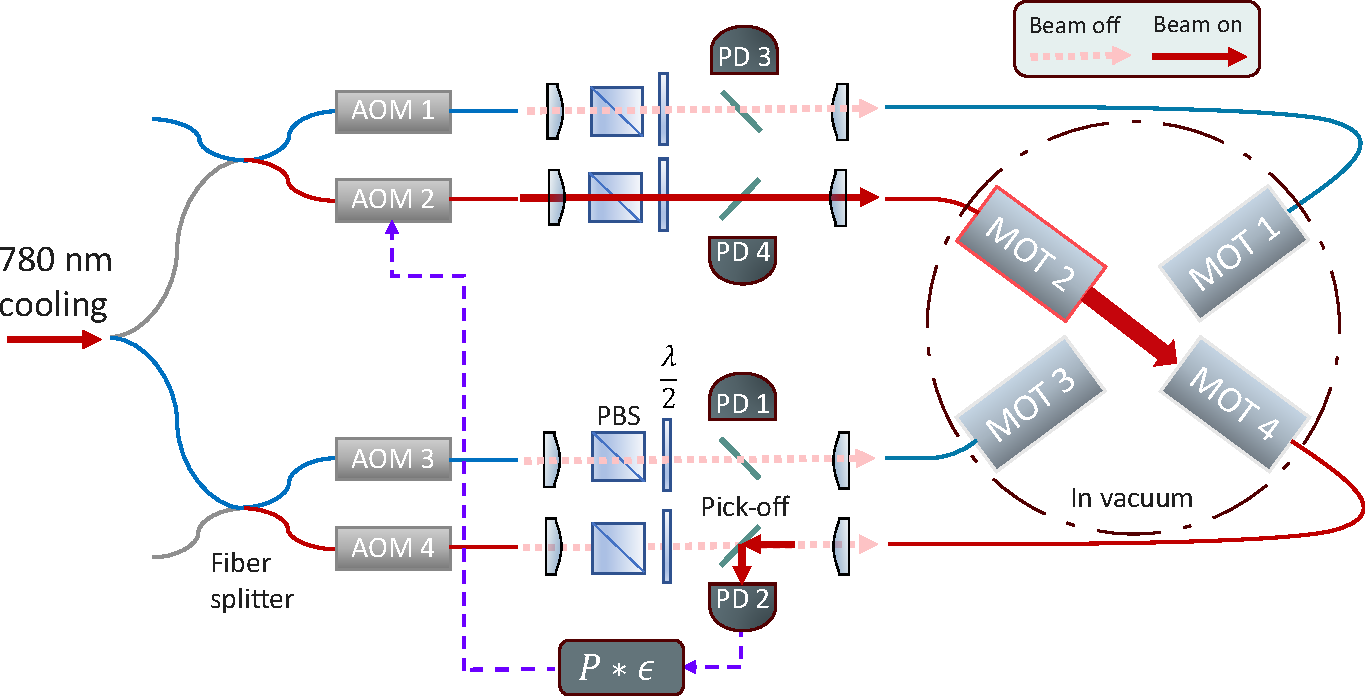
\includegraphics[width=0.9\textwidth]{Images/on_chip_mot_feedback.pdf}
    \caption{Schematic of the DC power stabilization for the on-chip
    MOT beams.}
    \label{fig:mot_feedback}
\end{figure}
This design choice was made for several reasons. Fiber splitter pick-offs could be used before the fibers going to vacuum, but the polarization state after the fiber AOMs drifts, and this is worsened with the addition of more fiber components. This means the light after the polarizer in vacuum for a given MOT beam will not correlate with the light measured at the pick-off port of the fiber splitter. Measuring the light after it has come back out of the vacuum  from the opposite fiber allows us to have a reliable proxy for the light after the polarizer of the MOT beam of interest. The reason for picking off in free-space is that we found fiber splitters to have uncorrelated output powers over time, i.e. the splitting ratio varies, such that the pick-off would not be reliable to the degree needed. While having high reliability, our approach has some shortcomings. Opposite MOT beams must be turned on one at a time during the feedback phase. This adds to the amount of time it takes to run feedback, as the beams can not all be adjusted in parallel. Typically, the feedback loop is run every time a MOT is loaded and takes $\sim 50$ ms, limited by averaging time as multiple measurements of the beam powers are recorded with the Sinara Sampler card to adjust the RF to bring the photodiode voltages to defined set points. The feedback loop for a particular beam exits when the photodiode voltage is within a defined tolerance of the set point.

\section{Trapping single atoms}
% finding single atom signals. dipole trap beam fixed wrt to 
% on-chip beams, necessity to shim the MOT to the correction position
% we don't need to be able to see the MOT on the SPCM, which is probably 
% explained by the emission of the MOT not coupling well to an SM fiber

\subsection{FORT formed with parabolic mirror}
% The red-detuned dipole trap. scattering rate. Raman scattering. 
% coupling into SM fiber, wonky feedback scheme.

The FORT used for trapping single atoms is formed by focusing 852 nm light with a 0.61 NA parabolic mirror, resulting in a $\sim0.8~\mu$m waist trap. As described previously, the focal pattern was prealigned to intersect MOT beams in the vacuum chamber (Fig. \ref{fig:parabolicfluorescence}).
\begin{figure}[!ht]
    \centering
    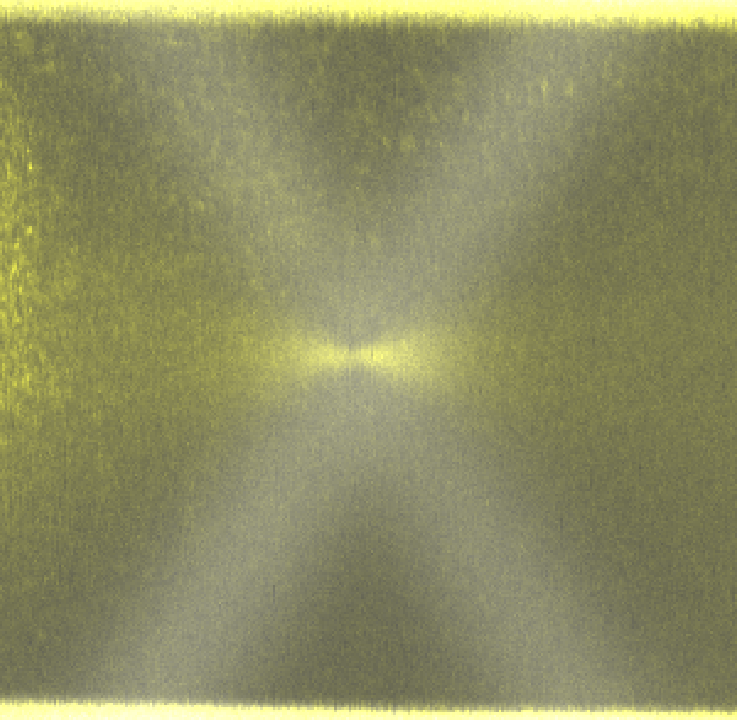
\includegraphics[width=0.5\textwidth]{Images/mirror_fluorescence_and_chip_beams_yellow.pdf}
    \caption{False-color image of the optical path of the FORT (yellow) and the on-chip MOT beams (grey) imaged with fluorescent emission from thermal Rb atoms in the chamber. The image is a combination of two separate images of the MOT beams and FORT path, both with 780 nm light, so that their pixel values could be scaled, clipped, and colored independently for optimal visualization.}
    \label{fig:parabolicfluorescence}
\end{figure}
For consistency in single atom trapping and the experiments to be described later, it is important to stabilize both the power and polarization of the light. Power stability is important to minimize DC drift of the AC Stark shift experienced by the atomic states, for example between $F=1$ and $F=2$ in the ground state during microwave rotations. Additionally, maintaining a high degree of linear polarization is typically necessary for achieving effective polarization gradient cooling (PGC), which can be hindered by the presence of a non-zero vector Stark shift introduced by non-zero ellipticity of the polarization\cite{chin2017polarization}.
% \begin{figure}[!ht]
%     \centering
%     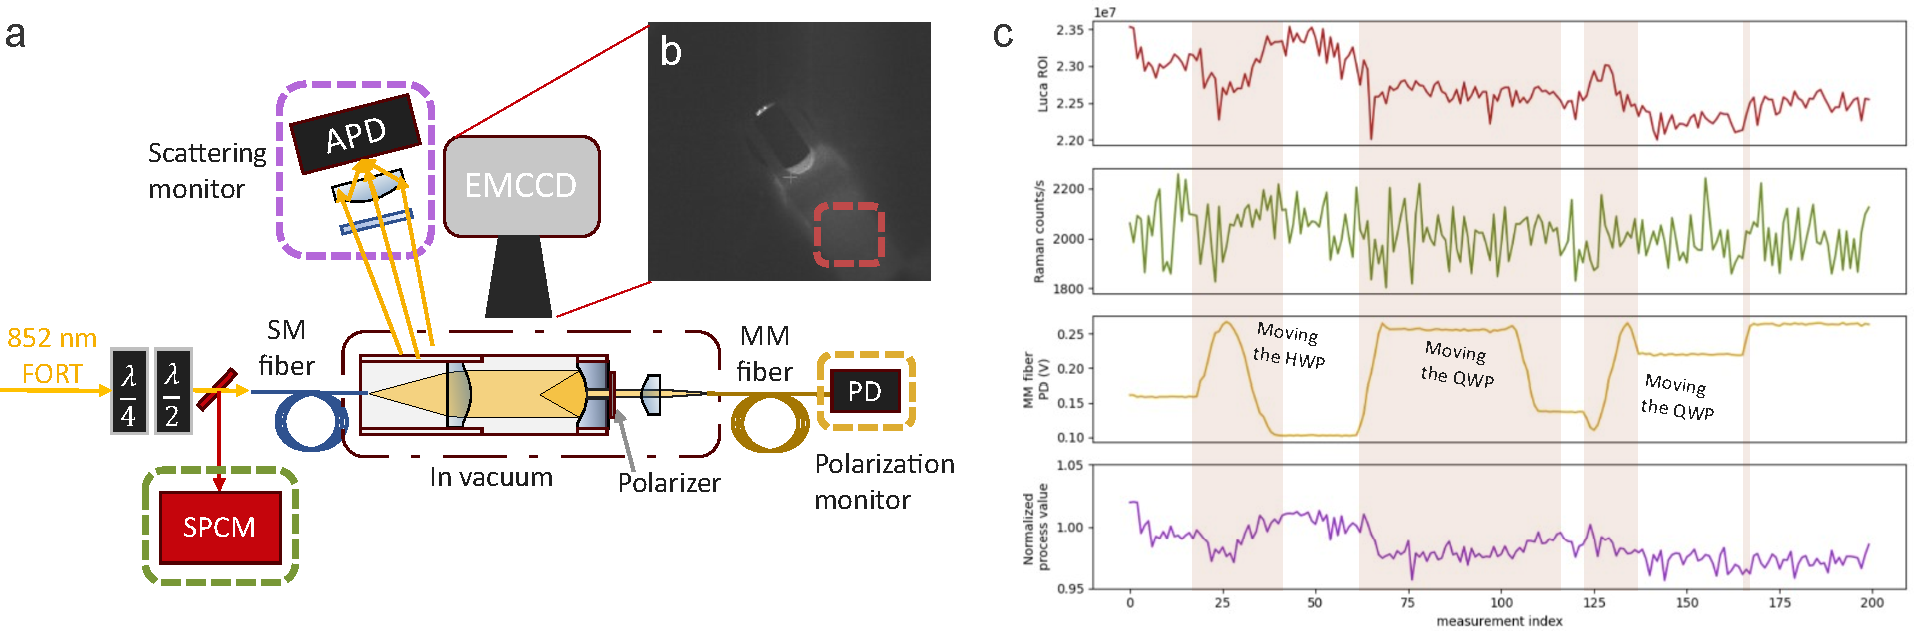
\includegraphics[width=0.9\textwidth]{Images/FORT_feedback.pdf}
%     \caption{Schematic of the polarization for the on-chip
%     of the 852 nm FORT light. DC power stabilization of the FORT is accomplished by measuring light scattered off surfaces in the chamber with an avalanche photodetector (not shown).}
%     \label{fig:fort_feedback}
% \end{figure}

% ?? \textbf{section needs to be reworked}

Because the FORT power is launched into the same SM fiber which carries out 780 nm photons emitted by trapped atoms, it is not possible to simply set a fixed polarization state before the fiber. For this reason, there is a hole bored through the parabolic mirror and a linear polarizer (Skight Optics) mounted behind the mirror, which allows some of the FORT light to pass through for optimizing the linearity of the polarization by monitoring light coupled out of the vacuum with a MM fiber. The power out of the MM fiber, measured with a photodetector (TTI), can be maximized by adjusting a quarter- and half-waveplate mounted in motorized stages (Thorlabs K10CR1). The polarizer transmission is typically observed to drift by not more than a couple of percent over the course of a day, so for now the polarization is not actively stabilized. We maximize the polarizer transmission "by hand" as needed by controlling the motorized waveplate mounts upstream of the SM fiber.

% The optimization algorithm used and results will be discussed in Sec. \ref{sec:FORTpolarizationOptimization}

\subsection{FORT power stabilization}

Stabilizing the optical power of the FORT is done by measuring light scattered off surfaces in the chamber, primarily the parabolic mirror tube, and feeding back to the FORT AOM as described in Sec. \ref{sec:fiber_AOM_power_stabilization}. An avalanche photodetector (APD, Thorlabs APD430A) with an asphere and 780 nm bandpass is mounted outside of the chamber's upper window, positioned for maximum signal from the scattered FORT light. SNR around 50 is typical for the science phase setpoint, and higher than this for the loading setpoint. Because the polarization is not stabilized as often as the power due to the associated cost to the experiment cycle rate, it was necessary to verify that the amount of scattering at the APD did not depend strongly on the polarization of the light. By programmatically rotating the motorized waveplates in the FORT path upstream of the SM fiber, we can maximize and minimize the transmission through the polarizer after the parabolic mirror, and compare with the scattering signal seen by the APD. For redundancy the scattering is also monitored with an EMCCD (Andor Luca). The results of these measurements are shown in Fig. \ref{fig:FORTfeedback}.

\begin{figure}[!ht]
    \centering
    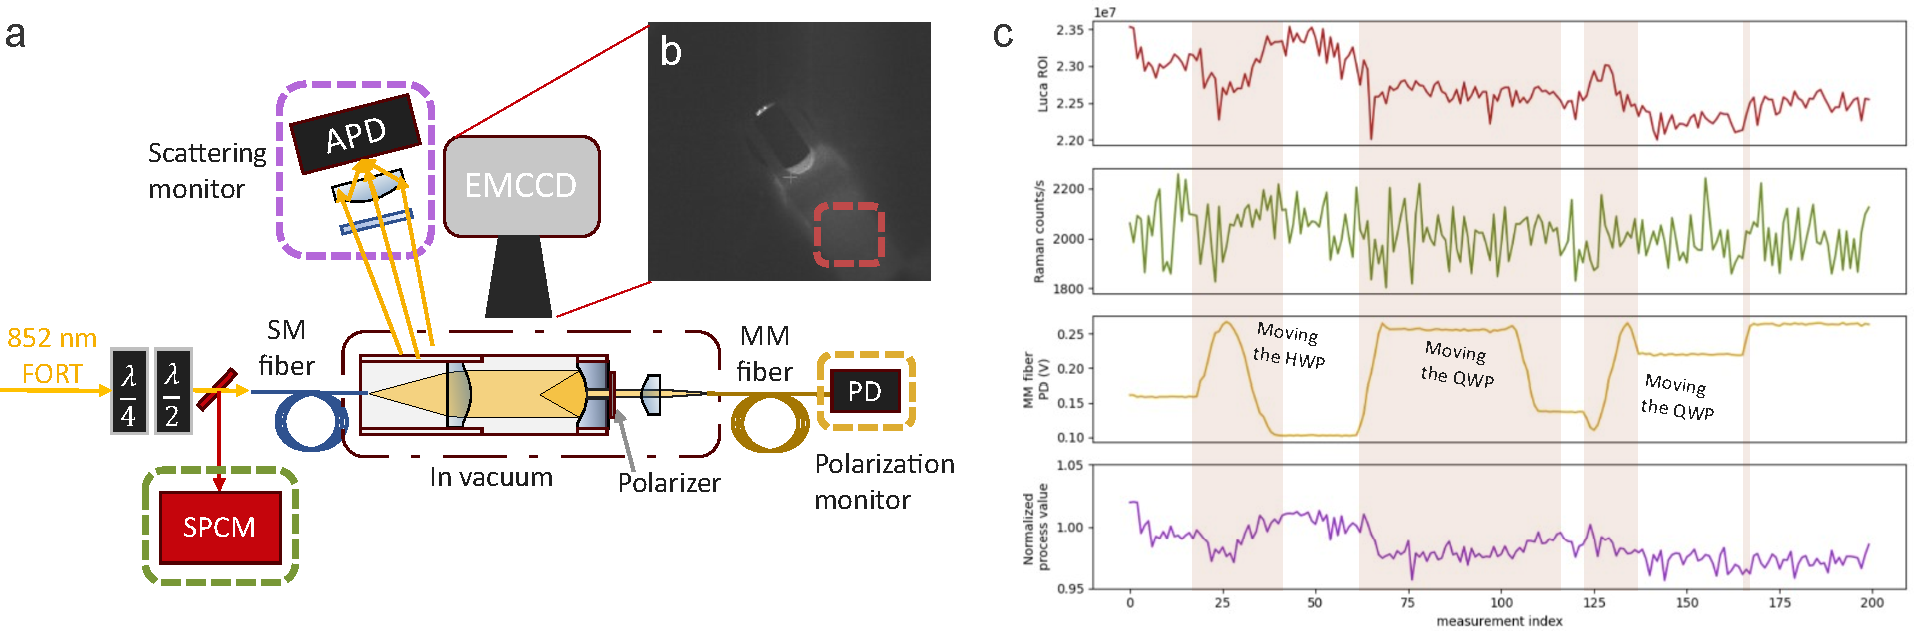
\includegraphics[width=0.9\textwidth]{Images/FORT_feedback.pdf}
    \caption{The feedback scheme for FORT dc intensity stabilization, shown schematically in (a). The inset (b) shows scattering from the FORT light on the Macor mirror tube in the chamber as viewed with an EMCCD. (c) Analysis of the extent to which the scattering monitored with the APD, which is used for dc stabilization of the FORT power, is dependent on polarization. The color of the data corresponds to the detectors outlined in the same color in (a).}
    \label{fig:FORTfeedback}
\end{figure}

the FORT light causes enough Raman scattering in the SM fiber at 780 nm, which can not be filtered out of from the light emitted by trapped atoms, and hence shows up during single atom readout.

The standard deviation of the Raman light from the SM fiber implies stability of the FORT power at the $1\%$ level, where shot noise can explain 0.7 of this. 

% The astute reader will have noticed that the photodetector's measurement of the FORT power can not distinguish between power and polarization drift, such that the relative rates of polarization and power drifts must be ascertained another way. Fortunately, the FORT light causes enough Raman scattering in the SM fiber at 780 nm, which can not be filtered out of from the light emitted by trapped atoms, and hence shows up during single atom readout, discussed later. When the polarization drifts during experiments, step (1) of the feedback will increase the optical power to bring the measured signal after the polarizer to the setpoint, thus increasing the light at the atoms beyond the intended set point. When this happens, the mean background during atom readout increases, and this can be monitored over many atom readouts in order to extract both the magnitude and rate of polarization drift. See Sec. \ref{sec:single_atom_readout} for relevant data.

% ?? say something about the estimated Raman rate here? maybe just the measured rate

% \subsection{FORT polarization optimization}\label{sec:FORTpolarizationOptimization}

\subsection{Single atom loading in steady-state MOT}
% Scanning the shim fields, monitoring SPCM counts to see atom-loading with
% the MOT and FORT on simultaneously, optimize the number of atoms loaded with
% M-LOOP from Vuletic group.

The first single atom signal in the network experiment was found by manually scanning the magnetic shim coil values and monitoring the counts recorded by a single photon counting module (SPCM) monitoring the 780 nm light out of the SM fiber. With the FORT turned on with an estimated 1 mK trap depth at the atoms, a sequence of jumps in the typical counts recorded by the SPCM in 10-15 ms exposure times heralds single atoms, shown in Fig. (\ref{fig:atoms_loaded_steady_state}) The hallmark of single atom loading is a bimodal distribution, meaning that there is sub-Poissonian atom loading: the mean number of atoms loaded is less than one, but there are never events with two or more atoms loaded (See Fig. \ref{fig:atom_histogram}).
\begin{figure}[!ht]
    \centering
    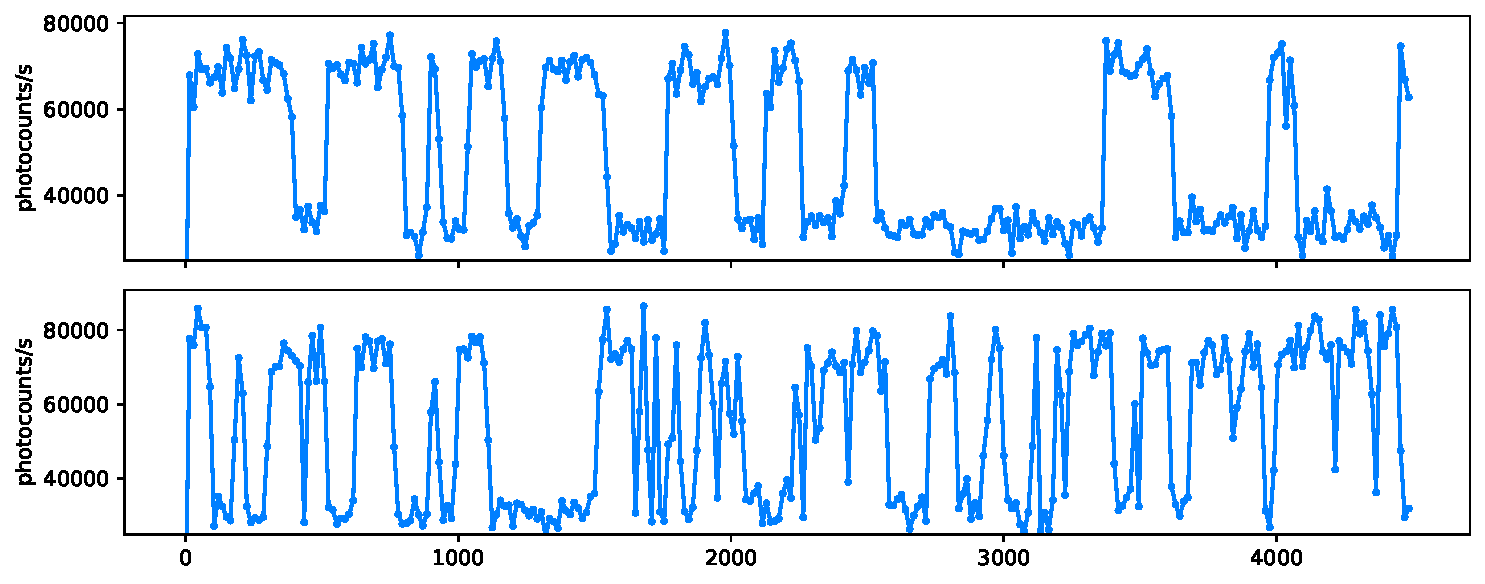
\includegraphics[width=0.9\textwidth]{Images/2024-06-21_atom_loading_with_continuous_MOT_time_series_loading_comparison_aspect0.02.pdf}
    \caption{Photon count rate as atoms enter and leave the FORT with the MOT loaded continuously. The top subplot shows clearly the bimodal nature of the signal, indicating that we load either zero or one atom. The lower subplot shows atoms coming and going more frequently, corresponding to a higher atom loading rate. Note that although the vertical axis is given
    as counts per s, the data collected in the lab is counts, 
    which is then divided by the exposure time for the SPCM here.}
    \label{fig:atoms_loaded_steady_state}
\end{figure}
We initially searched for single atoms by trying to first position the MOT to overlap the focal region of the FORT by watching for an increase in counts from the SPCM due to the collected MOT fluorescence. This proved both difficult and unnecessary, as the fluorescence signal from the MOT is extremely weak compared to that of a trapped single atom, which we attribute to the multi-mode emission pattern from the MOT not coupling well into an SM fiber. 

The data in the upper plot of Fig. \ref{fig:atoms_loaded_steady_state} corresponds to suboptimal loading parameters such that the FORT is likely not overlapped with the most dense part of the MOT, which explains why atoms can remain trapped for 100s of ms. The best single atom loading rate occurs when atoms are kicked out almost immediately after they are trapped, followed by a subsequent loading event.

The single atom loading rate is optimized using by tuning both coils and the power in each MOT beam, while loading the MOT continuously. This is done using an automated optimization routine which minimizes a cost defined as $-1$ times the number of atoms trapped within a 400 ms window. The optimization is done with ARTIQ, using M-LOOP, a machine learning optimization tool developed specifically for cold atom experiments \cite{Wigley2016}. Although single atom experiments in this work are done by loading the FORT over a fixed amount of time (see Sec. \ref{sec:fort_loading}) and then checking for the presence of an atom, the probability of loading an atom with that method reliably correlates with the loading rate observed in a steady state MOT. Moreover, this optimization method is at least an order of magnitude faster than optimization by loading the MOT and FORT for fixed times followed by checking for an atom. 

\subsection{Trap depth and vibrational frequencies}

The trap depth and characteristic Gaussian beam waist of the FORT can be measured by doing spectroscopy on the vibrational frequencies of trapped single atoms. Typically, one has an estimate of the trap depth given a measured or calculated beam size, beam power measured before the atoms, and a calculated polarizability of the atomic ground state. For the fiber-couple network node however, our estimate is limited to within a factor of two or so given that we can not directly measure how much 852 nm light couples into the SM fiber. Vibrational spectroscopy of the atom can be performed to allow us to back out these quantities.

A trapped atom in a red-detuned dipole trap can be modeled as a harmonic oscillator in a radially symmetric 3D potential well centered on the intensity maximum (see also Sec. \ref{sub:confine}) with radial and axial angular vibrational frequencies related to the trap depth and waist by
\begin{align}\label{eq:trapfreqs}
    \omega_{\rho} &= \frac{2}{w_0}\sqrt{\frac{U_0}{m}} \\
    \omega_z &= \frac{1}{z_R}\sqrt{\frac{2U_0}{m}}
\end{align}
where $w_0$ is the transverse $1/e^2$ intensity waist, $U_0$ is the trap depth, $m$ is the atomic mass, and $z_R=\pi w_0^2/\lambda$ is the Rayleigh range. The trap depth and waist can thus be extracted from spectroscopy of the vibrational frequencies. 

\begin{figure}[!ht]
    \centering
    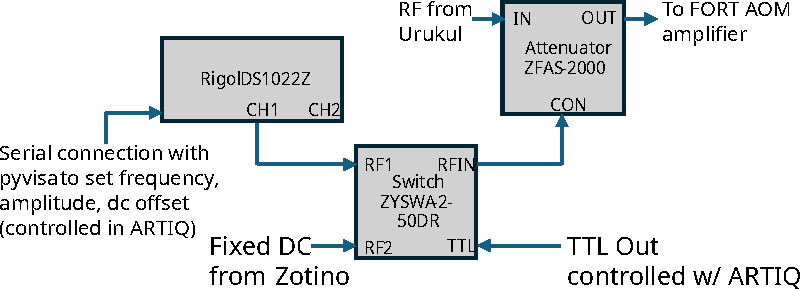
\includegraphics[width=0.9\textwidth]{Images/network_trap_frequency_electronics.pdf}
    \caption{Setup for switching between static and modulated trap for the trap frequency measurement. RF to the FORT AOM is controlled with a voltage controlled attenuator (VCA). The VCA is controlled with a DC voltage for atom loading and readout or modulated with DC + AC from a Rigol function generator between readouts, as determined by a switch.}
    \label{fig:networktrapfrequencyelectronics}
\end{figure}

The trap frequency measurement is done by loading and verifying the presence of an atom in the FORT (see Sec. \ref{sec:singleatomexperiments}), modulating the FORT sinusoidally for a fixed amount of time, and checking whether the atom is retained. A dip in the retention will show up when the FORT is modulated at twice the vibrational frequency. The electronics setup for modulating the trap light is shown in Fig. \ref{fig:networktrapfrequencyelectronics} and the measured vibrational spectrum is shown in Fig. \ref{fig:networktrapfrequencies}. We see two radial frequency dips owing to a slightly elliptical transverse trap profile which was first observed during the tapered fiber scans of the mirror focal intensity pattern (see Sec. \ref{sec:mirror}), though we have not come up with a definitive explanation of why the two radial resonances show different depths. 
\begin{figure}[!ht]
    \centering
    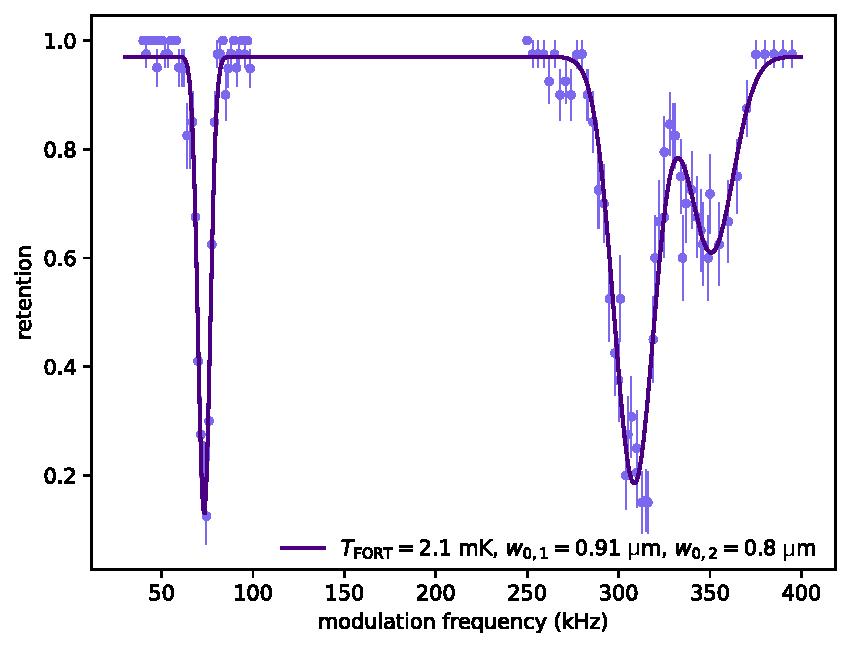
\includegraphics[width=0.9\textwidth]{Images/trap_frequency_experiment 15450.pdf}
    \caption{Vibrational spectroscopy of trapped atoms in the network experiment. The non-degenerate transverse resonances at high frequencies result from slightly different transverse waists in $x$ and $y$. The two axial resonances at low frequency are not resolved, showing up as a single resonance. The error bars are $1/\sqrt{N}$, with $N$ the number of atoms loaded per data point. The solid line is a fit to a sum of three Gaussians.}
    \label{fig:networktrapfrequencies}
\end{figure}
One possibility is that the modulation of the voltage controlled attenuator (see Fig. \ref{fig:networktrapfrequencyelectronics}) was not as strong for the higher frequency, though that frequency is still well within the 500 kHz control bandwidth. This can easily be checked by viewing the modulation on the FORT light.
    
We extract the trap depth and two beam waists by fitting the data to a sum of three Gaussians and assuming two equations for the transverse beam waist, for a total of three angular frequency relations. The fit frequencies are $(\omega_{\rho,1}, \omega_{\rho,2}, \omega_{z})/2\pi=($154.5 kHz, 175.3 kHz, 36.6 kHz$)$. The waist in the Rayleigh range expression in $\omega_z$ was replaced by the average of the two transverse waists as we do not resolve two axial resonances. Fitting the resulting frequency relations gives a trap depth of $2.1$ mK and transverse waists $w_{0,1}=0.91 ~\mu$m and $w_{0,2}=0.8 ~\mu$m.

\section{Single atom experiments}\label{sec:singleatomexperiments}
% The typical experiment sequence we use.    

\subsection{FORT loading, readout, and lifetime}\label{sec:fort_loading}
% Same as continuous MOT loading, but truncated to 500 ms, UV LED pulsed, MOT and FORT loaded, 
% MOT dropped, two readouts with science phase in the middle

% Fluorescence readout, contribution to background from FORT and MOT beams on continuously during readout, histogram, detuning of light, estimation of the power at the atoms.

\begin{figure}[!ht]
    \centering
    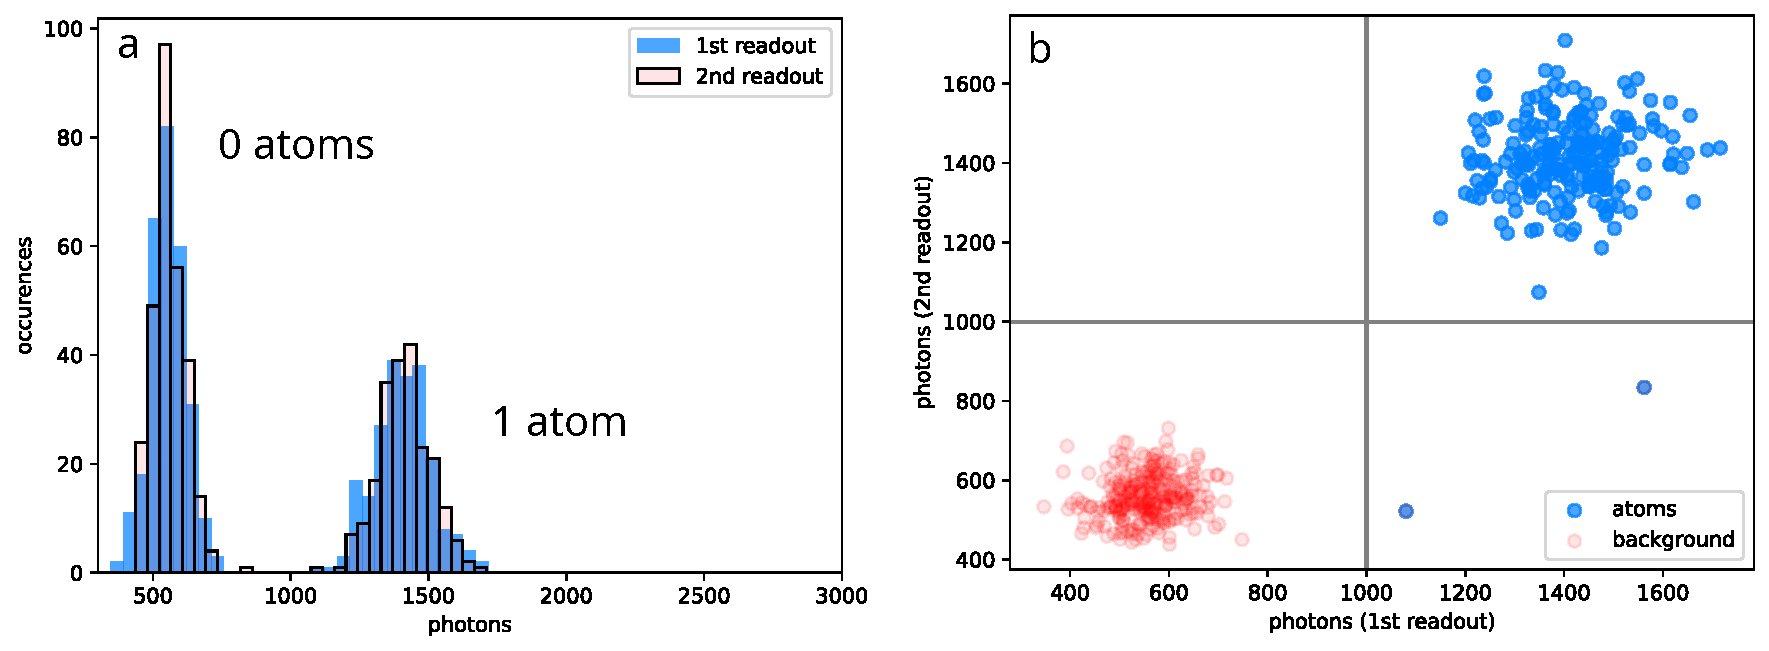
\includegraphics[width=0.9\textwidth]{Images/atom_histogram_and_scatterplot.pdf}
    \caption{Single atom readout data for the two experiment readouts or ``shots". The same data is shown \textbf({a}) as a histogram for each readout and (b) as a scatter plot, for a 14 ms exposure time and 3 ms holding time between shots. There is a clear absence of multi-atom loading events in (a), whereas the single atom loading fraction is 44$\%$ (b) shows that the fraction of atoms detected during the first shot which are also detected in the second, i.e. the retention fraction, is $99\%$.}
    \label{fig:atom_histogram}
\end{figure}

The presence of atoms in the second readout is used as the primary method of answering questions about what we have done to the atom. In specific, every question we want to ask is mapped onto ``with what probability do we expect an atom to be retained?"

The lifetime of the atoms in FORT has been measured by varying a delay between the readout while the atoms are in the trap, as shown in Fig. \ref{fig:atom_lifetime}. This lifetime is typically by the vacuum pressure, which determines the rate of collisions between the trapped atom with thermal atoms in the chamber. Lifetimes of $\sim10$ s are readily acheived by loading the MOT from a pre-cooled beam in a two-chamber setup\cite{Graham2022} rather than from background vapor as is done here, and up to over an hour by going to cryogenic temperatures\cite{Schymik2021}.
\begin{figure}[!ht]
    \centering
    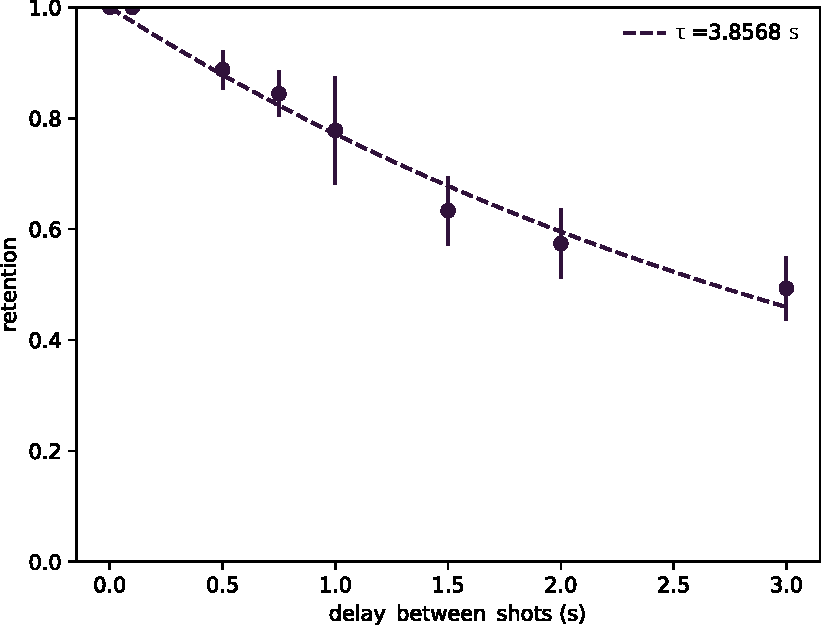
\includegraphics[width=0.5\textwidth]{Images/trap_lifetime_experiment 17951.pdf}
    \caption{Single atom lifetime in the FORT. The dashed line is a fit to a decaying exponential with decay constant $\tau$.}
    \label{fig:atom_lifetime}
\end{figure}

\subsection{Limitations to cycle time}
The single atom experiment described above provides the basic framework for most of the experiments described in this thesis. As such, any timing limitations intrinsic to this framework will affect the cycle rate we achieve. The dominant offender is the MOT loading phase, which typically takes 500 ms, depending on the pressure of background atoms in the chamber. Coming in second place is DC feedback to the MOT and FORT power to the atoms, as described in Sec. \ref{sec:fiber_AOM_power_stabilization}, which takes $\sim50$ ms. Lastly, the two atom readouts take $\sim10$ ms each. Enhancing cycle time is best achieved by atom reuse, so that we amortize the cost of loading the MOT over many experiments per loading event. This is of high importance for fast entanglement attempt rates (see Sec. \ref{sec:entanglementrate}).

\section{Qubit state preparation}

\subsection{Optical pumping and microwave rotations}

\begin{figure}[!h]
    \centering
    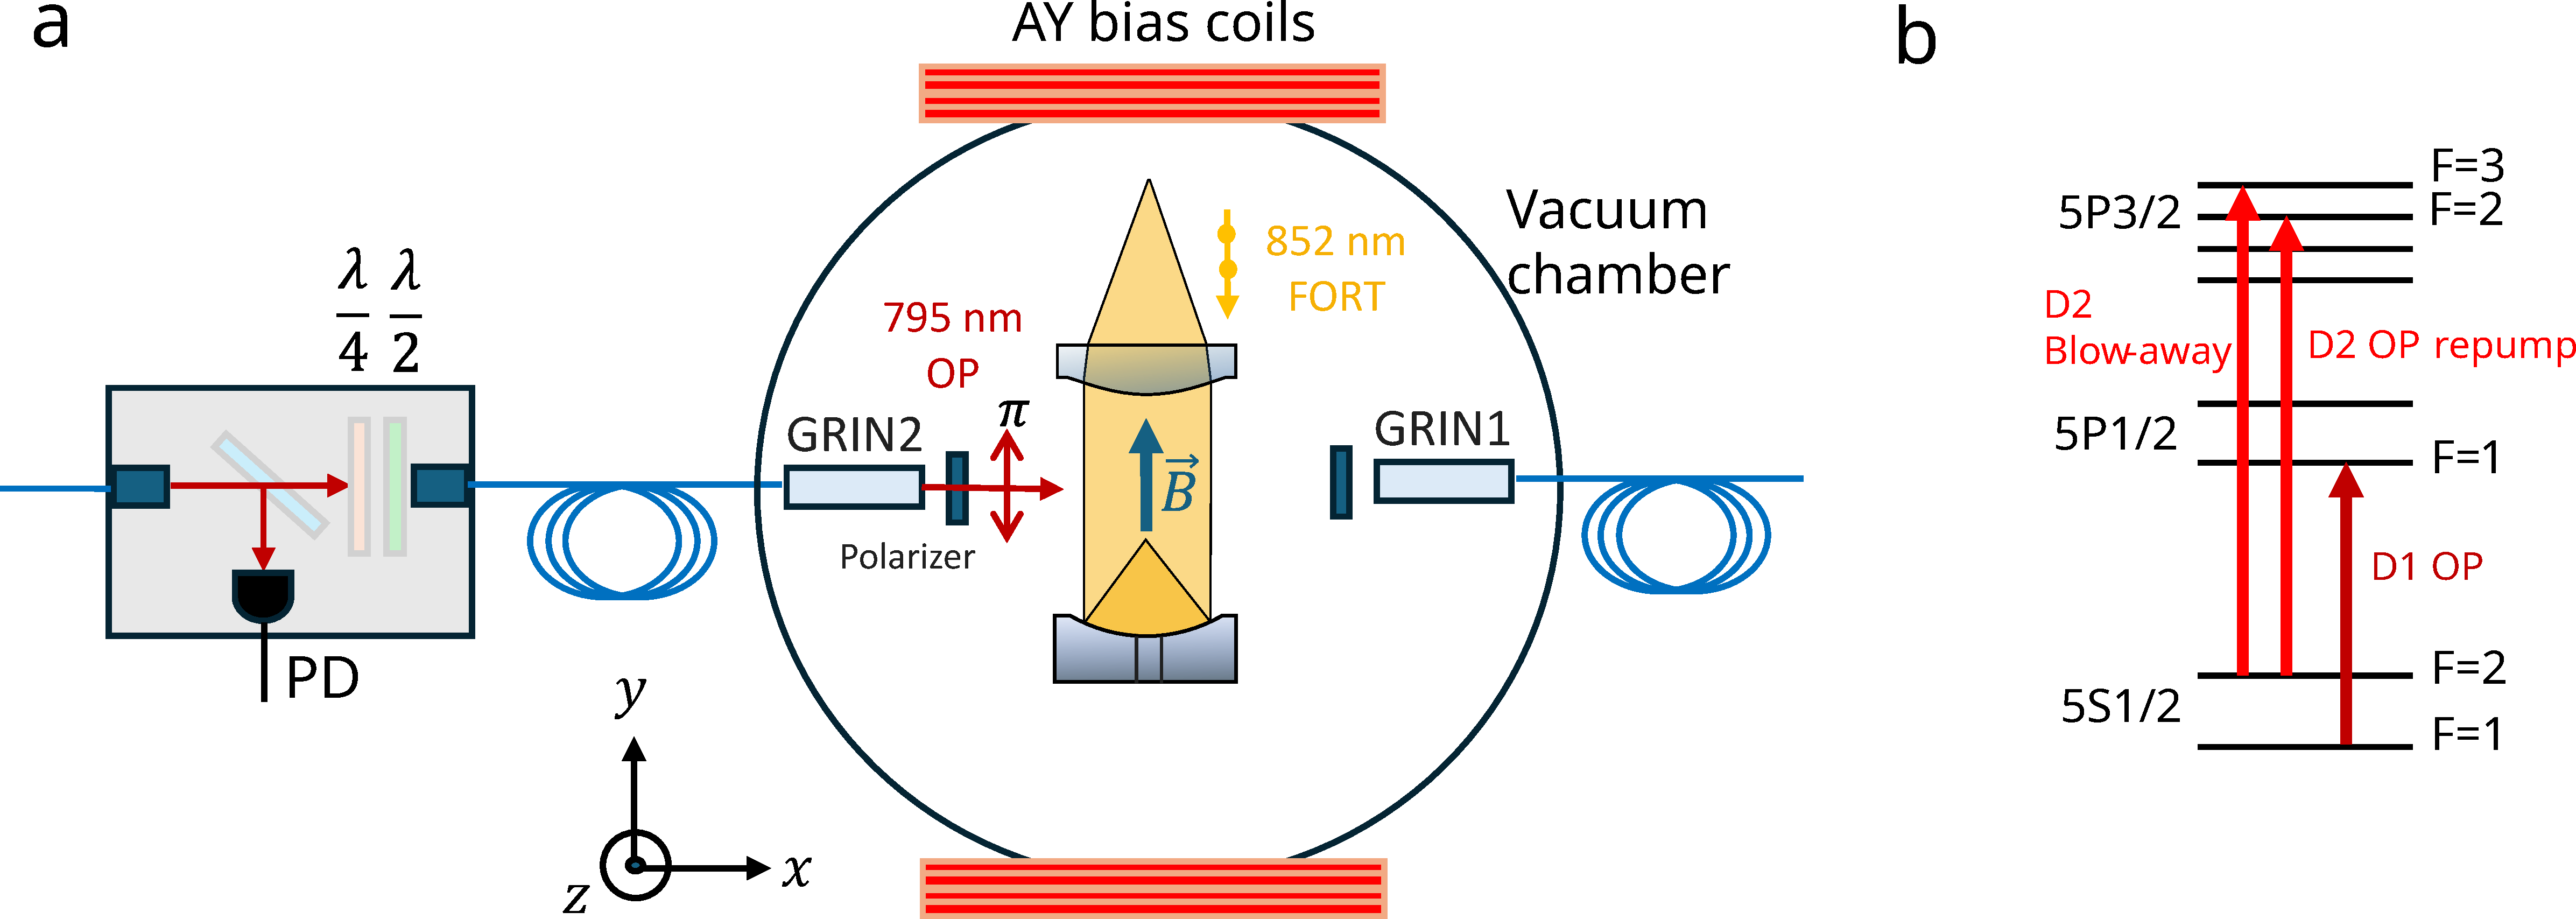
\includegraphics[width=0.9\textwidth]{Images/OP_setup.pdf}
    \caption{(a) The relevant components of the network node involved in optical pumping of the atoms and (b) the relevant energy levels, where only the hyperfine levels involved are labeled. PD is a TTI detector for monitoring pulse timing and power. Microwaves (not shown) for driving transitions between $F=1$ and $F=2$ states in the hyperfine ground manifold are polarized along $y$ and propagate along $-z$. The OP repump (not shown) is sent through the same paths as the MOT beams (either 1-6 or just 5 and 6) and blow-away light is sent through the free space MOT 6 path. Note that although the $\mathrm{D}1$ light is shown entering through GRIN2, we have more recently used GRIN1, for no particular reason, and may in the future alternate between the two during the optical pumping phase.}
    \label{fig:op_setup}
\end{figure}

The communication qubit state must be initialized into $\ket{F=1,m_F=0}$ for attempting
atom-photon entanglement generation. For optical pumping into this target state, we drive the $D_1$ transitions on $F=1 \leftrightarrow F'=1$ with linearly polarized light, for which the $m_F=0$ to $m_F'=0$ transition is dark. We typically apply a bias field of a few G parallel to the polarization of the light, which coincides with the axis of the parabolic mirror used for photon collection, as shown in Fig. \ref{fig:op_setup}. To avoid worrying about Stark shifts from the FORT, the optical pumping and FORT light are chopped on and off out of phase so that we only address the bare atomic states\footnote{It has been pointed out by M. Saffman that chopping the FORT at a rate comparable to the Zeeman splitting between $m_F$ states within $5S_{1/2},F=1$ can result in Raman-induced depumping from the target state.}.

Optical pumping fidelity is verified by driving the ground state clock transition $\ket{F=1,m_F=0} \leftrightarrow \ket{F=2,m_F=0}$ with microwaves delivered by an external horn, where full population transfer would indicate unity pumping fidelity. A typical microwave Rabi oscillation is shown in \ref{fig:microwave_oscillation}. For 3 ms of chopped optical pumping, we typically observe 90$\%$ fidelity. The observed Rabi oscillation is generally around 45 kHz, which is the expected order of magnitude given approximately 3 W microwave power emitted by the horn\cite{kwon2019rydberg}.
\begin{figure}[!hb]
    \centering
    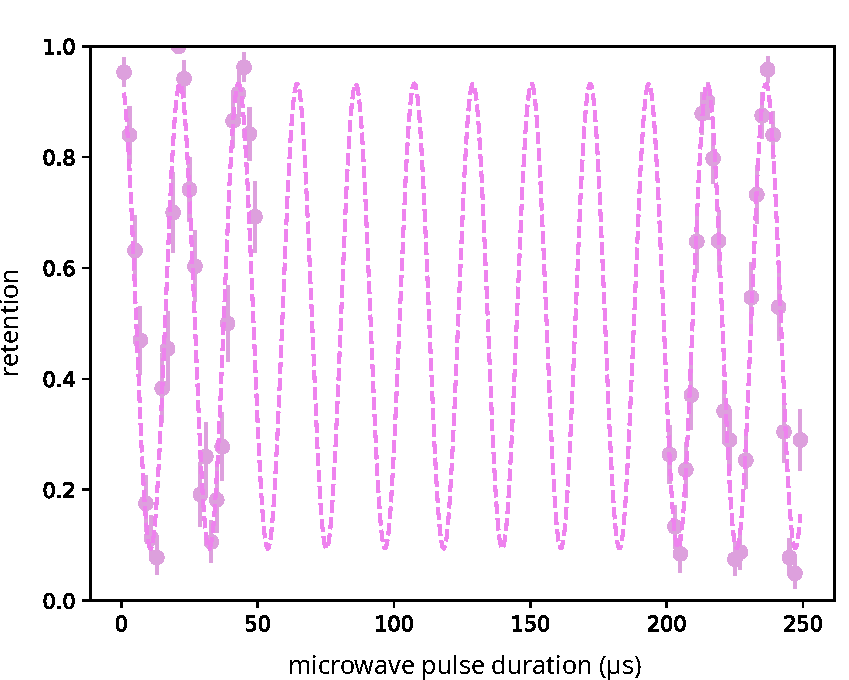
\includegraphics[width=0.5\textwidth]{Images/good_microwave_Rabi_experiment 19212_19211.pdf}
    \caption{Rabi oscillation between $\ket{F=1,m_F=0}$ and $\ket{F=2,m_F=0}$ driven resonantly by $\sim6.834$ GHz microwaves. The dashed line is a fit to an exponentially decaying cosine, indicating a Rabi frequency of $\Omega/2\pi=46.5$ kHz and a $1/e$ decay time of $0.096$ ms.}
    \label{fig:microwave_oscillation}
\end{figure}

The microwave system used has been adapted from the one used in \cite{Young2022thesis,kwon2019rydberg}, with minor modifications. The system, along with an RF line for use in the tomography of the atomic state, is shown in Fig. \ref{fig:microwave_system}.

\begin{figure}[!ht]
    \centering
    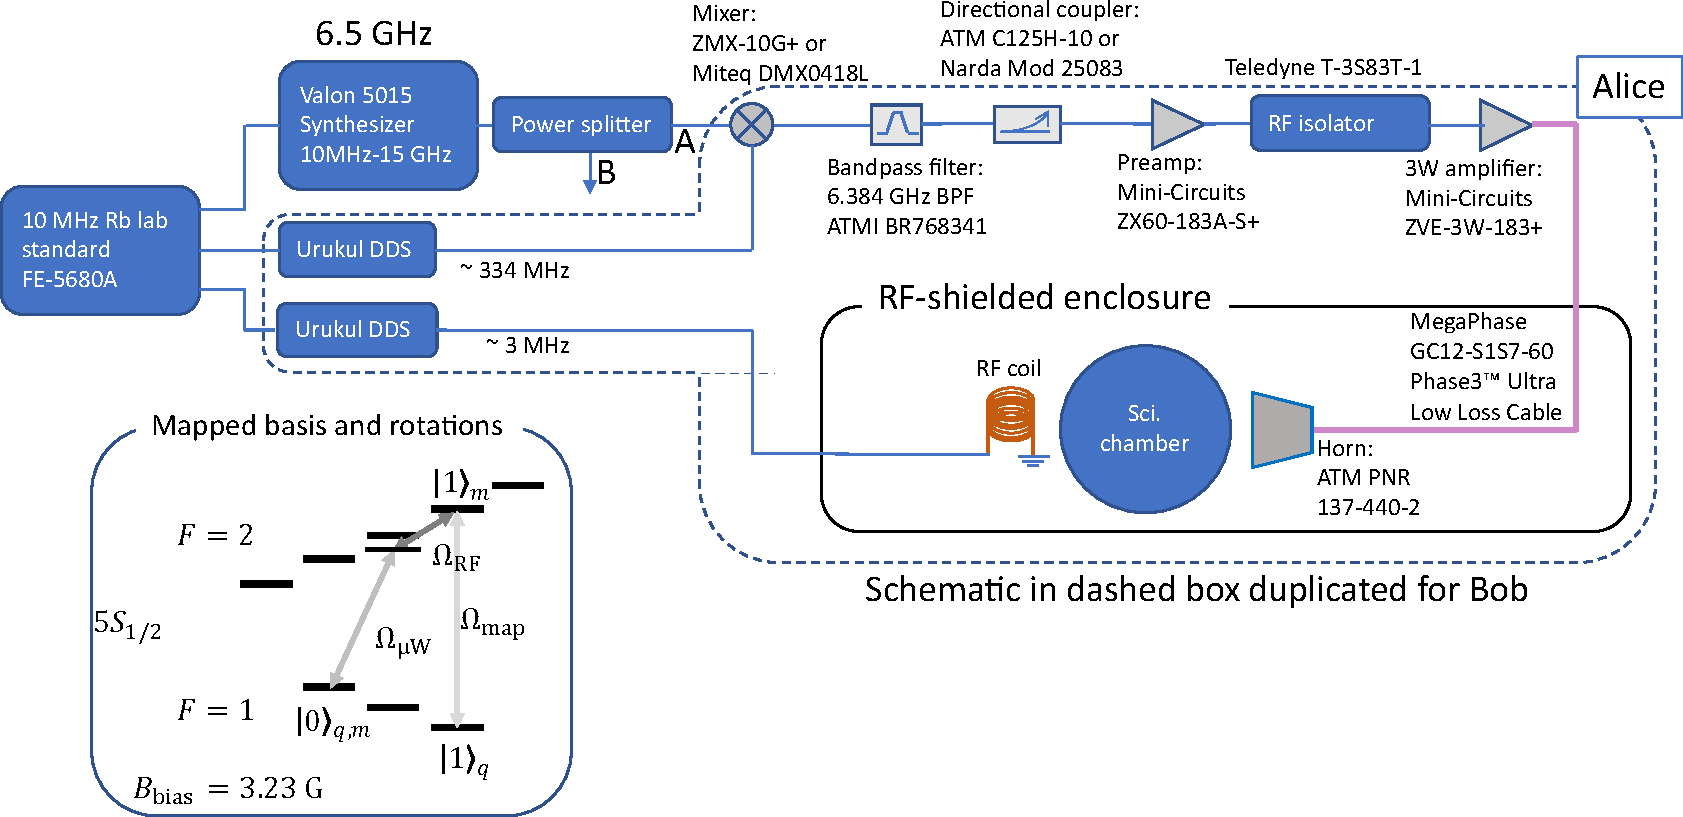
\includegraphics[width=0.9\textwidth]{Images/microwave_system_schematic.pdf}
    \caption{The microwave system used in the quantum network experiment and a (not yet implemented) RF line and coil planned to be used for two-photon rotations in the computational basis used for atom state tomography, as shown in the inset level diagram.}
    \label{fig:microwave_system}
\end{figure}

